\chapter{Description du Méta-Méta-Modèle Méta-HADL : M3}

	\section{Définition}
		
		Un Méta-Modèle permet à un modèle de s'auto-décrire. Il consiste à concevoir un modèle par lui même, à utiliser un modèle pour concevoir un autre modèle, à documenter un modèle et à comparer deux modèles.
		
	\section{Analyse}
		Afin de créer le Méta-HADL servant de base à notre HADL nous sommes partis du
		HADL et nous avons construit tous les éléments permettant de le définir
		correctement.
	
		\subsection{Meta-Entité}
			L'élément central servant de base à notre Meta-HADL et lui permettant de se redéfinir est Méta-Entité. A partir de cet élément nous allons tout construire.
			
			\begin{itemize}
				\item Relation : développée au paragraphe suivant.
				\item Entité : spécialisation d'une Méta-Entité.
				\item Attribut : Méta-Entité qui n'existe que pour appartenir à une autre
				Méta-Entité.
			\end{itemize}
		
		\subsection{Relation}
			Cet élément va permetre de définir les liens qui unissent les différents éléments :
				
			\begin{itemize}
				\item Est\_instance\_de : Spécialise une Méta-Entité en descendant d'un
				niveau dans les couches d'abstraction.
				\item Herite\_de : Spécialise une Méta-Entité en restant dans la même couche
				d'abstraction.
				\item Contient : Lie deux Méta-Entités en insérant l'une dans l'autre.
				\item Possede : Lie un Attribut à une Méta-Entité.
			\end{itemize}
			
			En plus de cela, elle possède deux attributs :
			\begin{itemize}
				\item From : Origine d'une relation.
				\item To : Destination d'une relation.
			\end{itemize}
			
	\section{Diagrammes}
	
		Voici comment se structure notre Méta-Méta-Modèle Méta-HADL.
	
		\begin{figure}[!h]
			\centering
			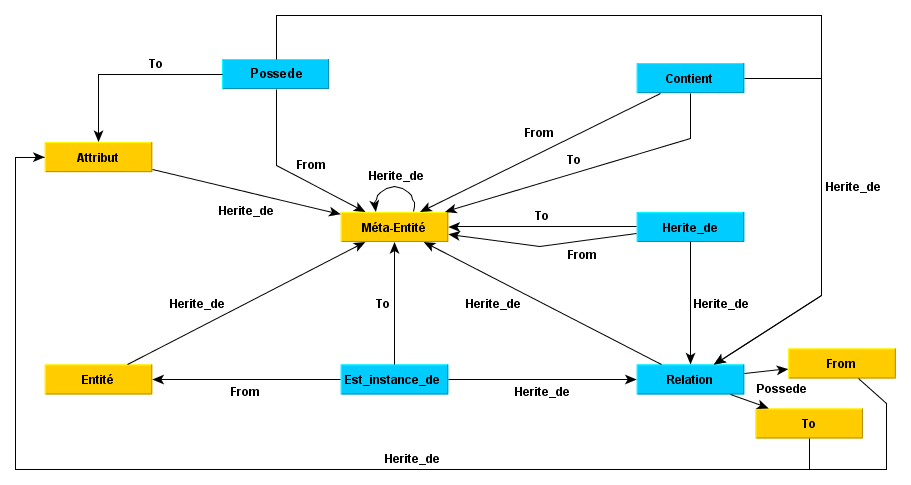
\includegraphics[scale=0.5]{../images/m3.png}
			\caption{représentation du M3}
		\end{figure}
	
\clearpage